\chapter{Methodology}
\section{General Considerations}

For this work an algorithm is designed both for Lennard-Jones calculation and the management of the different programs that were used throughout the protocol; an overview of the workflow is displayed in Figure \ref{fig:flowchart1}.
The protocol employed in this work starts with a COF selection from the CoRE COF database. The CIF file is then imported, and data were extracted by the algorithm. A single layer is extracted from the structure and placed at the bottom of the simulation box. The geometry of the polymer is kept the same throughout the process. If the charges were missing, the single-layer is passed through an external charge equilibration routine (see \ref{sec:charge}). Then the list of x and y displacement vectors to be tested, in this case, a 25x25 evenly spaced grid over the unit cell, is generated and distributed among threads. Each of the threads then computes the approximate distance between the two sheets at which the Lennard-Jones (LJ) potential cancels for the x,y point.  A two-stage convergence is used for this purpose to increase the speed and cheapen the calculations : first the COF top layer is be displaced by 0.1 unit-cell at every iteration and the LJ potential is computed. When the energy reaches negative values, the COF starts the process over starting from the last distance to yield positive energy using a 0.01 displacement at each iteration. The starting distance $z_0$ for the z PES is the last point to yield positive energy using that second displacement step. From that initial distance $z_0$, 10 points spaced by 0.01 unit-cell were defined, and the $z_0$ point is stored. For each x,y,z grid-point a copy of the single-layer is generated and shifted by the x,y,z offset. All the offsets were defined in cartesian coordinates, hence a z-shift does not affect the x,y offset. The Lennard-Jones interactions are computed by a built-in function of the algorithm. The two structures were then exported under CIF format to be fed in LAMMPS (for LJ and Coulombic calculations), and XYZ format for calculations with DFTB+ and CP2K's implementation of xTB (for tight-binding approximation calculations). The single point energy were obtained with xTB and DFTB+ using bash scripts and run on the FIDIS EPFL cluster. The main program then collects the energies, find the grid-point with the lowest energy associated and generate the structure associated with that grid-point as CIF file to be finally optimized using CP2K's DFT function.



Each COF is studied using a naive structure (theoretical bond-angles and bond-lengths) and using this same structure relaxed using CP2K's geometry and cell optimization in order to assess the need to relax the structure before going to the calculations of the PES.

\begin{figure}\centering\scalebox{0.8}{
\begin{tikzpicture}[node distance = 1.5cm, auto]\centering
    % Place nodes
    \node [cloud] (start) {start};
    \node [block,below of=start] (db) {COF database};
    \node [block,below of=db] (import) {Import new COF and isolate single layer};
    \node [decision, below of=import](has_chg) {Charge assigned ?};
    \node [block,right of=has_chg] (charges) at (3.5,-6) {Charge equilibration}  ;
    \node [block, below of=has_chg] (xy) at (0,-7) {Pick an x,y offset};
    \node [block, below of=xy] (ELJ0) {Find a $z_0$ offset where $E_{LJ}\simeq0$};
    \node [block, below of=ELJ0] (struct_gen) {Generate a structure using the given x,y,z offset ($z_0<z$)};
    \node [block, below of=struct_gen] (LJ) {Compute Lennard-Jones Potential}; % resulting from interactions between the atoms of the two sheets
    \node [block, below of=LJ] (export) {Export generated structure};
    \node [decision, below of=export] (zover) at (0,-14) {z PES computed ?};
    \node [decision, below of=zover] (allover) at(0,-17.5) {All PES computed ?};
    \node [block,below of=allover] (funcall) at (0,-22) {Process structure though LAMMPS, xTB, DFTB+};
    \node [block, below of=funcall] (collect) {Collect energies and find minimum};
    \node [block, below of=collect] (DFT) {Final optimisation with DFT};
    \node [cloud, below of=DFT] (end) at (0,-25) {end};
  

  \path [line] (start) -- (db);  
  \path [line] (db) -- (import);
  \path [line] (import) -- (has_chg);
  \path [line] (has_chg) -- node {no} (charges);
  \path [line] (has_chg) -- node {yes} (xy);
  \path [line] (charges) -- ++(0,-2.5) -- ++ (-2.4,0);
  \path [line] (xy) -- (ELJ0);
  \path [line] (ELJ0) -- (struct_gen); 
  \path [line] (struct_gen) -- (LJ);
  \path [line] (LJ) -- (export);
  \path [line] (export) -- (zover);
  \path [line] (zover.west) -- ++(-2.2,0.0) -- ++ (0,5.5) -- ++(1,0);
  \path [line] (zover) -- node {yes} (allover);
  \path [line] (allover) -- node {yes} (funcall);
  \path [line] (allover.west) -- ++(-3,0) -- ++ (0,12) -- ++(1.8,0);
  \path [line] (funcall) -- (collect);
  \path [line] (collect) -- (DFT);
  \path [line] (DFT) -- (end);
  %\path [line] (funcall.west) -- ++(-0,-0.1) -- ++(-1.2,0.0) -- ++ (0,7.6) -- ++(1.2,0)  ;
  %\path [line] (funcall.west)  -- ++(0,+0.1) -- ++(-1,0) -- ++ (0,4.4) -- ++(1,0)  ;
  %\path [line] (DFT.west) -- ++(-2,0) -- ++ (0,13.5) -- ++(2,0)  ;
\end{tikzpicture}}
\caption{\textit{Workflow of the project}}
\label{fig:flowchart1}
\end{figure}


\section{Lennard-Jones}
%The Lennard-Jones potential is a classical approximation of non-binding interactions where interaction potential between two elements i and j is given by :
%$$E_{LJ}=4\epsilon_{ij}\left[\left(\frac{\sigma_{ij}}{r_{ij}}\right)^{12}-\left(\frac{\sigma_{ij}}{r_{ij}}\right)^{6}\right]$$
%where and $\epsilon_{ij}$ and $\sigma_{ij}$ are pair-specific parameters. 
%The positive part sands for the repulsion that results from the Pauli exclusion principle and the negative one for the coulombic attraction. The exponents were chosen for computational simplicity.
To asses the complexity of the phenomenon involved in the stacking process of COFs, the Lennard-Jones potential is used as a first approach to simulate the Van der Waals interactions. The parameters used were the Universal Force Field parameters from Rapp\'e et al. \cite{rappe_uff_1992}. Since these parameters are element-specific, a mixing rule is needed to combine the parameters. In our case, the Lorentz-Berthelot mixing rules were used\cite{lorentz_ueber_1881}%, as it is the simplest and most widely used one. It reads as follow:
%$$ \sigma_{ij}=\sqrt{\sigma_i\sigma_j}   $$ and $$ \epsilon_{ij}=\frac{\epsilon_i + \epsilon_j}{2}$$
%where indices i denote an element-specific parameter for element i, and indices $ij$ a pair-specific parameter. $\sigma_i$ and $\epsilon_i$ are the distance to $E_{LJ}=0$ from the nucleus and the depth of the well respectively.
%The parameters used are the Universal Force Field  ones
%, which is among the simplest classical approximations in computational chemistry
The tail correction used here is the truncated-shifted correction :
$$E_{LJ}^{corr}(r)=E_{LJ}(r)+E_{LJ}(r_{cut})$$
Where $E_{LJ}^{corr}(r)$ is the corrected potential, and $r_cut$ is the cutoff radius; it ensures a smooth potential at cutoff.

\section{Charge Calculations}
\label{sec:charge}
For the experimental structures (naive bond angle and bond length), no charges were provided and where hence computed for a single sheet using the charge equilibration from EGULP subroutine \cite{kadantsev_fast_2013}. This method is also based on the Universal Force Field's parameters. The core principle behind this method is to use a second-order Taylor expansion, truncated to the second-order, of the charge dependant energy ($E(Q)$)\cite{rappe_charge_1991} :
%$$E_A(Q)=E_{A0}+Q_A\left(\frac{\partial E}{\partial Q}\right)_{A0}+\frac{1}{2}Q_{A0}^2\left(\frac{\partial^2 E}{\partial Q^2}\right)_{A0}$$
This parametrization makes this problem computationally cheap by avoiding to go through a long and tedious quantum processing of the system and hence fast charge equilibration.

Calculations were performed on a single sheet to exclude Coulombic interactions between layers.

% Unfortunately, this method was not robust enough and showed some unphysical behaviors, among others yielding strongly asymmetric charge distribution in a symmetric system or yielding positively charged Fluorine in fluorinated benzene. This indicates that the systems under study here need to be dealt with more advanced techniques to obtain the equilibrated charges. Hence 

The charges were also computed using DFT with the parameters detailed in section% \ref{sec:dft}

The charge density was partitioned using either the Hirshfeld method \cite{hirshfeld_bonded-atom_1977} or the Density Derived Electrostatic and Chemical (DDEC) charge method \cite{manz_chemically_2010}.

An in-depth analysis of the charges as computed by DFTB+ is also performed to asses the strength of the interactions between layers in the repartition of charges. This may enable one to estimate the correlation between charge distribution and stacking and hence the necessity to recompute the charges for every configuration or not. 



\section{Coulombic Potential and Ewald Summation}

%The Coulombic potential is given by :
%$$E_c=k_e\frac{q_iq_j}{r_{ij}}$$
%where $k_e$ is the Coulomb's constant, $q_i$ and $q_j$ the charge of the atoms i and j respectively, and $r_{ij}$ the distance between the two atoms. 
%Since the potential converges slowly in periodic systems, it is important to take into account the long-range interactions. A natural way to do so would be to use a very high cutoff but it would increase the computational cost drastically. To tackle this problem, one can take advantage of the periodicity of the system and compute separately the short-range interactions by summing them in real space and sum the long-range interactions in reciprocal space: this is known as the Ewald summation, which is a special case of the Poisson summation. The charge density is split as follow :
%$$\rho_i(r) = \rho_i^S(r)+\rho_i^L(r)$$
%where $\rho_i^S(r)$, the short-range function is as follow
%$$\rho_i^S(r) = q_i\delta(r-r_i)-q_iG_\sigma(r-r_i)$$
%and $\rho_i^L(r)$, the long-range function :
%$$\rho_i^L(r)=q_iG_\sigma(r-r_i)$$
%with 
%$$G_\sigma=\frac{1}{(2\pi\sigma^2)^{3/2}}exp\left[-\frac{|r|^2}{2\sigma^2}\right]$$
%The substitution above is equivalent to adding and subtracting a Gaussian function around each point charge, described by a Dirac delta function. This will shield long-range interactions in the short-range function and is corrected by the long-range function to maintain a correct description of the physical system.
%We then integrate the short-range function in real space and the long-range in reciprocal space.
Since our problem is a periodic system, the convergence of the Coulombic potential is achieved using the Ewald summation\cite{lee_ewald_nodate}. For this project, LAMMPS (Large Scale Atomic/Molecular Massively Parallel Simulator)\cite{plimpton_fast_nodate} is used for its implementation of the Particle-Particle-Particle-Mesh Ewald Summation (PPPM) \cite{hockney_computer_1981} , with a threshold of $10^{-6}$ $kcal/mol$.
Only interactions between two designated sets of atoms, here the two layers, were computed and hence neglecting the intra-layer interactions
% To be able to grasp the principle of the two following technics, it is important to first go through the principle that is the foundation of almost all newly developed technics: the Density Functional Theory. It mostly lies on the Hohnenberg-Kohn theorem that states that : 

%\textit{In a finite, interacting N-electron system with a given particle-particle interaction, there exists a one-to-one correspondence between the external potential v(r) and the ground state-density $n_0[v](r)$. In other words, the external potential is a unique functional of the ground-state density, $v[n_0](r)$, up to an arbitrary constant}\cite{ullrich_time-dependent_2011}. 

%With :
%$$n_0[v](r)=\sum_i|\Psi_i(r)|^2$$

%This equivalence simplify greatly the calculations and enabled computational chemistry to start tackling problems of a complexity that was before out of reach. The difficulty now resides in finding an efficient functional to compute the energy and other system properties.



% It lies on the equivalence between treating $N$ one-electron wavefunction $\Psi_i$ and one $N$ electron density function $n(r)$ with :
%where the summation is done over the $i$ electrons.
%It is based on the fact that a non-degenerate ground state of a $N$ electron system is fully determined for a given external potential, and hence :
%$$V_{ext} \leftrightarrow n(r)$$
%The first Hohnenberg-Kohn theorem goes further and state that a unique functional of the density function $n(r)$ exists and yield the energy of the system.
%The second Hohnenberg-Kohn theorem state that the true density function of the ground state is the one that minimizes the energy.
%Together these theorems are the foundation of DFT calculations.

For the CP2K relaxed structures, the charges were provided as computed by DFT in the two-layer structure provided.

 
\section{Geometry, Frequency, Non-bonding - Tight Binding method (GFN2-xTB)}

GFN2-xTB is a Tight-Binding approximation with atom-specific parametrization. For the purpose of this project, the CP2K delvopment version of this algorithm was used with the D3 dispersion correction and the SPME (Smooth Particle Mesh Ewald) summation, the Hessian matrix is estimated using the Broyden mixing scheme using the last 8 steps and was alternated with the Direct Inversion in the Iterative Subspace \cite{pulay_convergence_1980}\cite{pulay_improved_1982}\cite{shepard_comments_2007}. The threshold for SCC conversion used is $10^{-6}$ and the D3 correction for dispersion%It is mostly designed for vibrational analysis, geometry optimization and non-covalent interactions (the latest being the one of interest here).
%The theory it relies on reads as follow, starting from the total energy :
%$$E=E_{el} + E_{rep} + E_{disp} + E_{XB}$$
%with $E_{rep} $ the repulsion energy, $E_{disp}$ the dispersion energy and $E_{XB}$ the halogen bonding and $E_{el}$ the electronic potential is based on a corrected third-order-truncated Taylor expansion of the Hamiltonian :
%$$E_{el}=\sum_i^{occ}n_i\braket{\Psi_i|H_0|\Psi_i}+\frac{1}{2}\sum_{A,B}\sum_{l(A)}\sum_{l'(B)}p_{l}^Ap_{l'}^B\gamma_{AB,ll'}+\frac{1}{3}\sum_A\Gamma_{A}q_A^3-T_{el}S_{el}$$
%The first order therm is simply the energy associated with each electron in its Molecular Orbital, the second order and third order term are the SCC contribution taking only in account diagonal terms and the additional term $T_{el}S_{el}$ is the electronic thermal-entropic terms.
 
 %$\Psi_i$ is the valence Molecular Orbital with occupation $n_i$, $H_0$ the zero-order Hamiltonian, $q_A$ the Mulliken charges of atom $A$, $\Gamma_A$ the derivative of the Hubbard parameter $\eta_A$,$l$ and $l'$ are the electronic shells of atoms $A$ and $B$ respectively and $p_l^A$ the charge distribution on atom $A$'s shells with angular momentum $l$  and $\gamma_{AB,ll'}$ is a Coulombic space-dependant damping factor.

%xTB is run on CP2K's development version


\section{DFTB+}
The Density Functional-Based Tight Binding (DFTB) implemented on DFTB+ program is a more heavily parameterized method. Like xTB, it relies on an expansion around the density-functional energy but uses atomic parametrisation for the electronic Hamiltonian diagonal terms (element-specific) as well as for the off-diagonal ones (pair specific).
For this process, were used two sets of parameters : the 3ob-3-1 (parametrisation for Organic and Biological System) set \cite{kubillus_parameterization_2015}\cite{lu_parametrization_2015}\cite{gaus_parameterization_2014}\cite{gaus_parametrization_2013} and the Matsci-0-3 \cite{frenzel_semirelativistic_nodate} (parametrisation for Material Sciences) set for COFs containing Boron (COF-1 and COF-5). The two sets of parameters were compared for a COF were both sets could be used.
The static grid-point calculations were performed with a self-consistent Hamiltonian, with a force and self-consistency threshold of $10^{-5} a.u$, the Broyden mixer is used, and the k-points were set to x,y,z=\{1,1,1\}, the D3 method using the Becke-Johnson damping factor and including the Hubbard derivatives is used for dispersion correction and damped in the special case of Hydrogen to mimic Hydrogen-bonding.

The cell and geometry optimization is performed using the same parameters except with a lower threshold for the forces and SCC: $10^{-6}$. 

%It is based on the spin-polarized Hamiltonian below :
%$$\hat{H}_{\mu\nu}^\sigma = \braket{\phi_\mu|\hat{H_0}|\phi_\mu}+\frac{1}{2}S_{\mu\nu}\sum_C\sum_{l''\inC}(\gamma_{Al,Cl''}+\gamma_{Bl',Cl''})\Delta q_{C_{l''}}$$
%$$\pm \frac{1}{2}S_{\mu\nu}\left(\sum_{l''\in A}W_{All''}m_{Al''}+\sum_{l''\in B}W_{Bll''}m_{Bl''}\right)$$
%The first term being the non-SCC Hamiltonian, the second term is the SCC contribution,



\section{Density Functional Theory}
\label{sec:dft}
%Density Functional Theory is a technique relying on the physical equivalence of a set of $N$ one-electron wavefunction $\Psi(r)$ and the sum of its position dependent module $n(r)$, the density function. A functional is then applied to the density function to extract observables as the energy. It was here used as the last stage of our process to obtain the reference COF stacking starting from each technique's guess to asses its accuracy. The parameters used were the same as for the charge equilibrations.

The charge calculations using DFT were performed with PBE (Perdew$-$Burke$-$Ernzerhof), a nonempirical GGA (Generalized Gradient Approximation) functional and Self-Consistency Field (SCF) is enforced using DIIS minimizer (Direct Inversion in Iterative Subspace) \cite{pulay_convergence_1980}\cite{pulay_improved_1982}\cite{shepard_comments_2007} with a threshold of $10^{-6}$. The DFT-D3 correction term for dispersion forces (London Forces) is used and set to include the $9^{nth}$ order term since these play a key role in the non-bonding interactions which will determine the optimum stacking. For all elements, including Hydrogen, a Gaussian Double-Zeta function is used for the basis set \cite{vandevondele_gaussian_2007} to mimic accurately polarisation.

The geometry and cell optimisations were performed with the same method as for the charge optimisation, no symmetry constrains nor external pressure were applied and with the Broyden–Fletcher–Goldfarb–Shanno (BFGS) optimiser, a type of steepest descant optimizer.

\section{COF sample}
In order to assess the different phenomenons that intervene in the stacking process of Covalent Organic Frameworks, a chemically and structurally diverse set of COFs was chosen. they are represented on Figure \ref{fig:struct}. The two first ones are among the first synthesized COFs by Cot\'e et al., the first is made by cyclic condensation of boronic acids. The second one by condensation of boronic acid and di-alcool. The third fourth and fifth by triazine cyclic condensation and the last one by imine condensation. The first fourth are flat COF the fifth one is non-flat because of the methyl groups and the sixth one is slightly V-shaped because of the steric hindrance of the Hydrogens between the benzene and the pyrene; this curvature induces a strain on the pyrene and break aromaticity.

\begin{figure}[H]

%\caption[A floating table]{Structures of the COFs under study}

\centering
\begin{tabular}{cc}
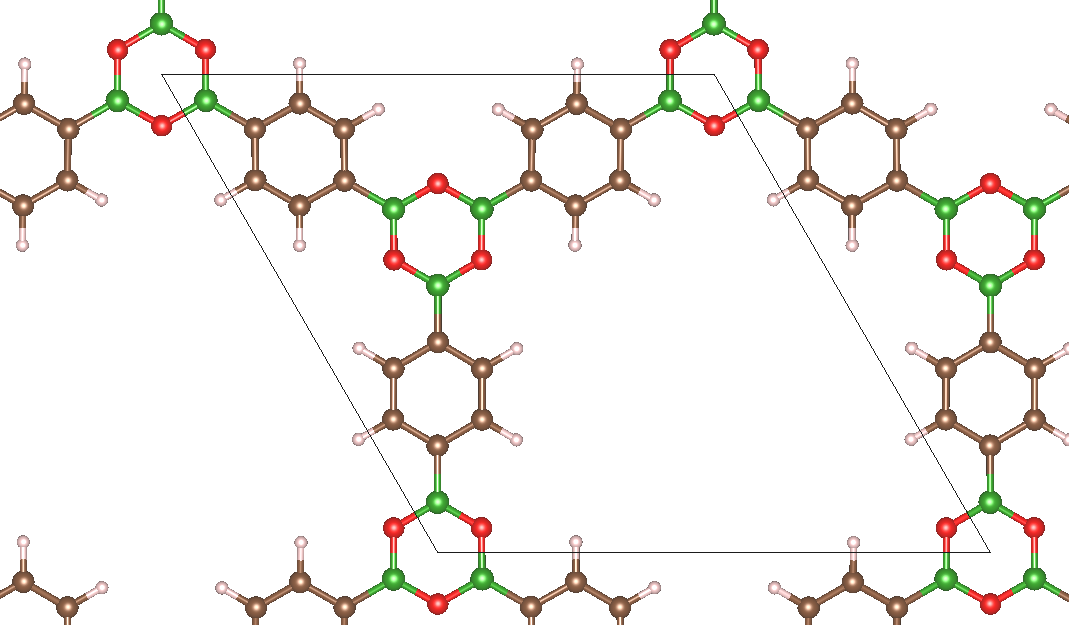
\includegraphics[height=4cm]{images/05000.png} & 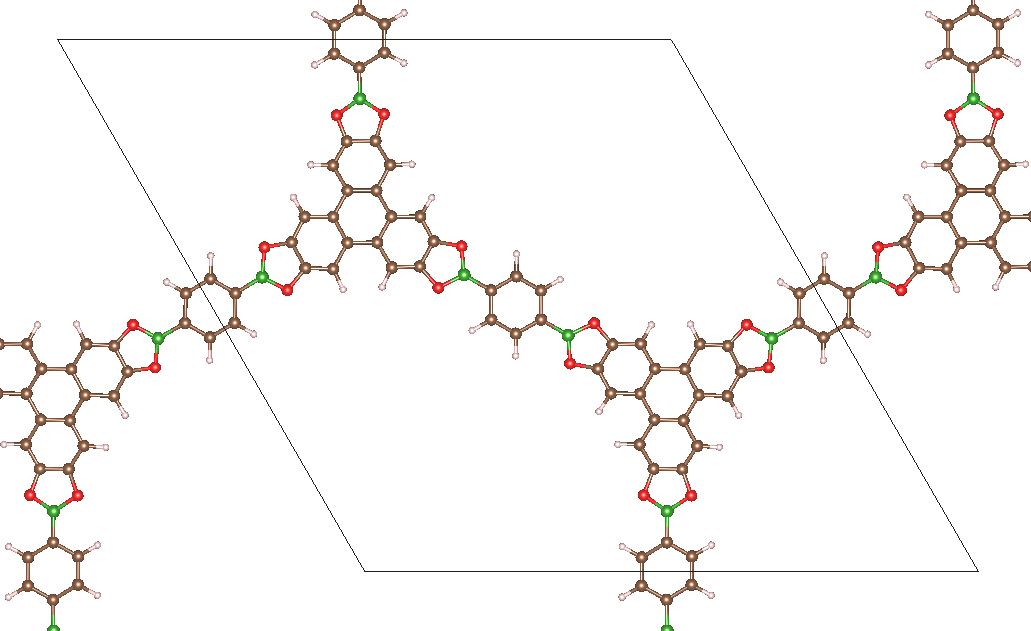
\includegraphics[height=4cm]{images/050001.png} \\ 
\textbf{05000N2}\par\medskip & \textbf{05001N2}\par\medskip\\
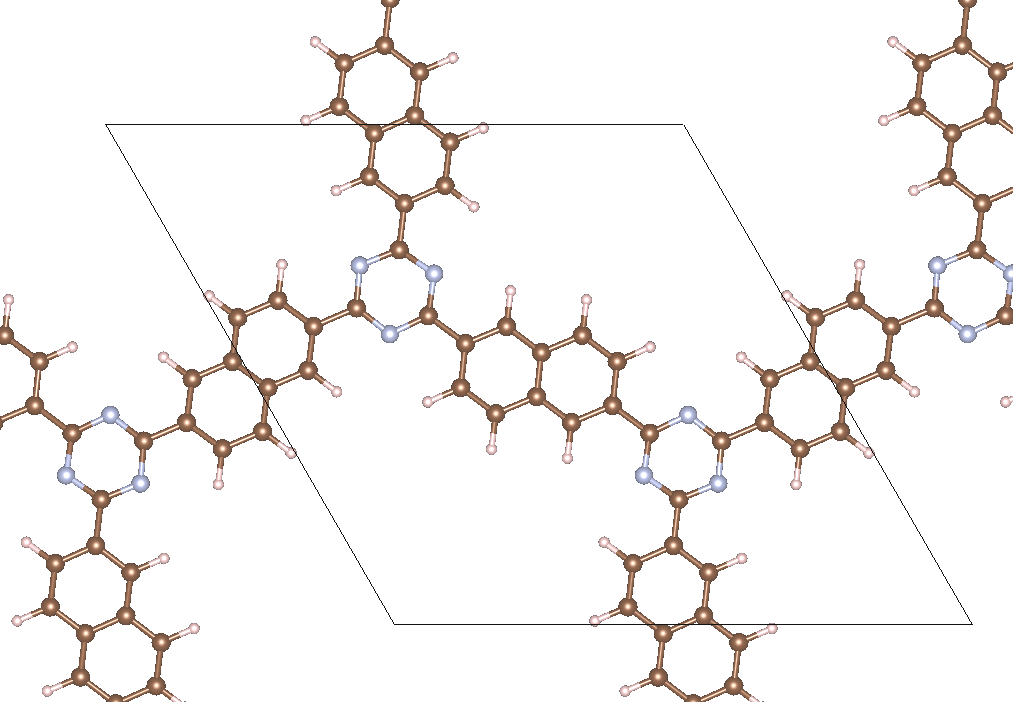
\includegraphics[height=4cm]{images/10000.png} & 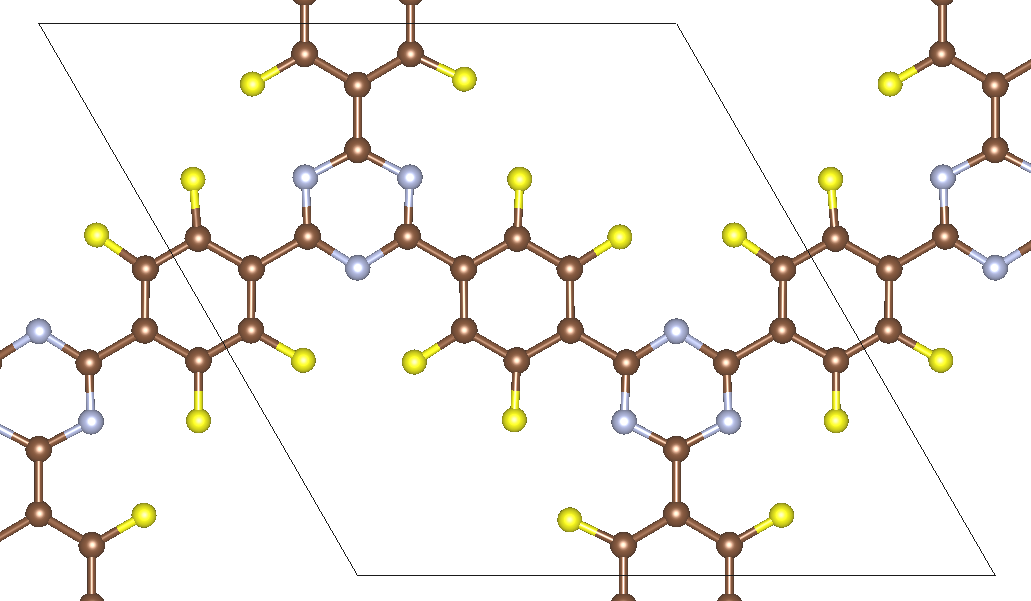
\includegraphics[height=4cm]{images/13000.png} \\
\textbf{10000N2}\par\medskip & \textbf{13000N2}\par\medskip\\
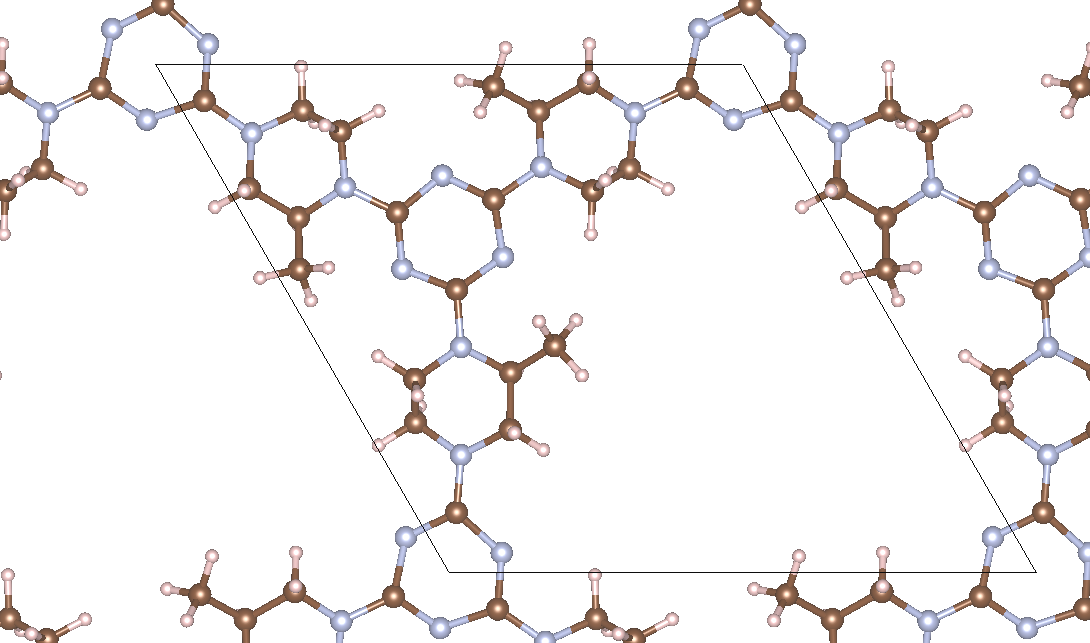
\includegraphics[height=4cm]{images/17120.png} & 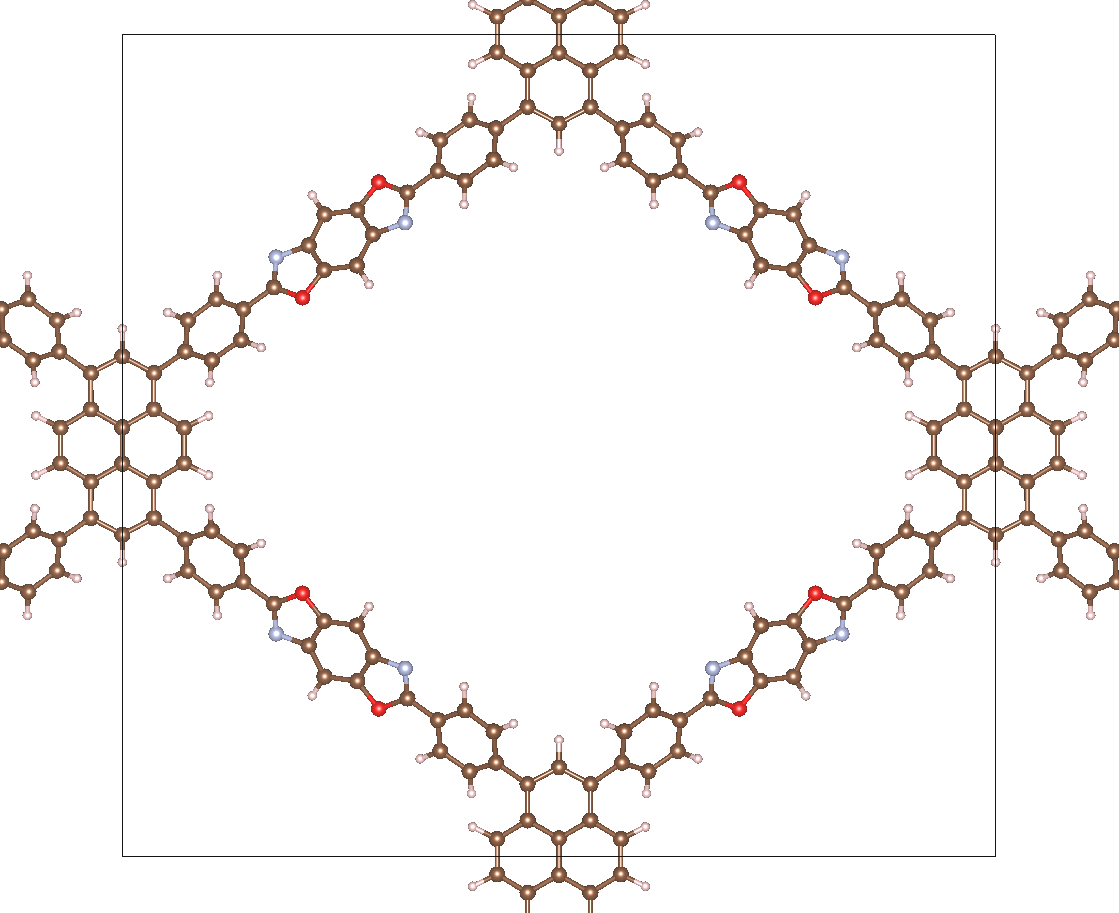
\includegraphics[height=4cm]{images/18112.png} \\ 
\textbf{17120N2}\par\medskip & \textbf{18112}\par\medskip\\
\end{tabular}
\caption{Structure of COFs studied in this work; from left to right and top to bottom; Carbon in brown, Oxygen in red, Hydrogen in white, Boron in green, Nitrogen in blue, Fluorine in yellow}
\label{fig:struct}
\end{figure}
